

There are many methods to create something new, but they all begin with an idea that needs to be realized. The path to realization in some cases can involve simply building the final project; however, with aerospace engineering that is not usually the case. In order to achieve the end goal, much planning is needed. An idea is formed, researched, designed, and then built. With many aerospace projects, designing cutting-edge technology requires accurate physical modeling in order confirm the feasibility of a design and examine the effects of changes. Therefore, the field of aerospace simulation and modeling is a large and extensive field. It is one which is constantly changing and expanding as computing power becomes exponentially stronger. The boom in computing power has opened the door to this thesis. \par

\begin{figure}[ht]
    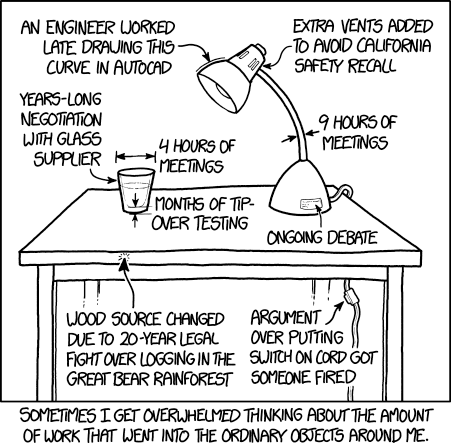
\includegraphics[width=.45\textwidth]{figures/work.png}
    \centering
    \caption[Example of various engineering design tasks]{Example of various engineering design tasks \cite{xkcd}}
    \label{fig:xkcd}
\end{figure}


\section{Motivation}





\indent Computational Fluid Dynamics (CFD) is the field of study which deals with creating simulations of fluids. This is a critical part of aerospace design and analysis. Viscous fluid dynamics are completely described through the Navier-Stokes Equations.

\Needspace{12\baselineskip}
\begin{equation}
    \label{eqn:navier_1}
    \partial_t u_i + R u_j \partial_j u_i = -\partial_i \rho + \nabla^2 u_i + E_i 
\end{equation}
\begin{equation}
    \label{eqn:navier_2}
        \partial_j u_j = 0  
\end{equation}
\(u_i\) = Velocity components (m/s)\footnote{Throughout this thesis, repeated indices mean sum over that index.} \newline
\(R\) = Reynolds number \newline
\(\rho\) = Pressure (Pa) \newline
\(E_i\) = External Forces (N) \par



\indent The Navier-Stokes equations, seen in Equations \ref{eqn:navier_1} and \ref{eqn:navier_2} in the incompressible form \cite{navier_eqns}, have no known closed-form solution without making simplifying assumptions. They must be solved numerically and, to increase their accuracy, call for increases in computational power to match. CFD is currently an accepted and reliable industry tool for analysis across many disciplines. As computers continue to get stronger, more complicated modeling techniques can be used for unique and diverse scenarios. \par

\indent A large part of aerospace research involves states of matter where the particle density is low. Atmospheric re-entry of spacecraft, objects in Low Earth Orbit (LEO), planes flying at extremely high altitudes, and interactions with plasma all involve fluids whose particles are relatively far apart from each other. The relative spacing between particles can be measured through the Knudsen number, seen in Equation \ref{eqn:Knudsen}. \par

\Needspace{7\baselineskip}
\begin{equation}
    \label{eqn:Knudsen}
    Kn = \frac{\lambda}{L}
\end{equation}
\(Kn\) = Knudsen number \newline
\(\lambda\) = Mean free path \newline
\(L\) = Characteristic length \par


\begin{figure}
    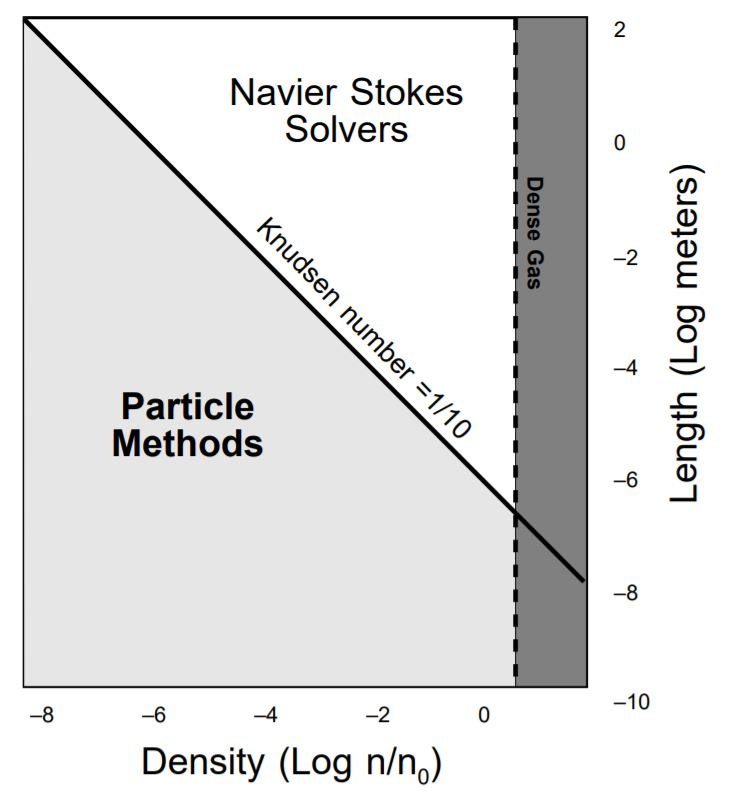
\includegraphics[width=.55\textwidth]{figures/navier.JPG}
    \centering
    \caption[Appropriate Simulation Models by Knudsen number]{Appropriate Simulation Models by Knudsen number \cite{navier} \(n_0\) is the density of air at standard temperature and pressure at sea level}
    \label{fig:navier}
\end{figure}


\indent The mean free path is a measure of how far particles move before interacting with other particles and the characteristic length is a description of the basic length scale of the problem at hand. The ratio of the two (the Knudsen number) shows their relative differences and, therefore, quantifies whether continuum is a good assumption for that fluid. When the Knudsen number is very low ( \(\sim10^{-3}\) ) the particles collide much more often than they move the characteristic length, which means that a continuum assumption is valid. However, as seen in Figure \ref{fig:navier}, when the Knudsen number is large ( \(\sim10^{1}\) and up ) the continuum assumption, and by inference the Navier-Stokes equations, are no longer valid. One reason they are no longer valid is because in the Navier-Stokes Equations (\ref{eqn:navier_2}), where the divergence of the velocity is zero, the density of the fluid remains constant, and therefore is incompressible. High Knudsen number fluids are almost always compressible and therefore the divergence of their velocity is non-zero. \par


\indent There is another equation which can solve high Knudsen number problems. This is the Boltzmann equation, shown in kinematic form for elastic interaction of particles in a plasma by Equation \ref{eqn:boltzmann} \cite{boltzmann}. It is based upon the statistical distribution of particles and their momentum. \par


\Needspace{3\baselineskip}
\begin{equation}
    \label{eqn:boltzmann}
    \frac{\partial f_i}{\partial t} + \vec{v_i} \cdot \frac{\partial f_i}{\partial \vec{r}} + \vec{F_i} \cdot \frac{\partial f_i}{\partial \vec{v_i}} = \sum_j \int_0^\infty \int_0^{2\pi} \int_0^\infty  [ f_i(v_i^\prime) f_j (v_j^\prime) - f_i (v_i) f_j (v_j) ] g_{ij} b \text{d} b \text{d} \epsilon \text{d} v_j
\end{equation}
\(f(v)\) = Particle distribution function \newline
\(i \: \text{and} \: j\) =  \(i\)th and \(j\)th species \newline
\(v\) = Velocity  \newline
\(F\) = Force acting on the particle \newline
\(\prime\) = Functions for post-collision \newline
\(g_{ij}\) = Initial relative velocity between particles \newline
\(b\) = Impact parameter \newline
\(\epsilon\) = Azimuth angle \par

\indent The Boltzmann Equation can be solved for a few select unique fluid scenarios. These scenarios usually involve knowing the entirety of the initial state, being in a near equilibrium state or being in a near vacuum environment \cite{boltzmann_solved}. In order to model other more complicated scenarios the Boltzmann Equation is nominally solved numerically, like the Navier-Stokes equations. To solve the equation numerically is a large task, considering the triple integral, the unknown way to find an accurate function for the particle distribution, and the curse of dimensionality. It would follow that a discretion of the Boltzmann Equation would be helpful. This is where a particle-based code begins to make sense. \par

\indent The most basic algorithm for a particle-based simulation is to keep track of every particle in the domain and calculate each collision depending on the particles' relative distances. While this algorithm, called Molecular Dynamics (MD), is a valid algorithm, computers are not strong enough currently to create meaningful results from such a computationally heavy solution. This is where Direct Simulation Monte Carlo (DSMC) comes into play. DSMC was introduced in 1963 \cite{dsmc_speed}, one year before the computer language BASIC was created \cite{basic}. Back then, DSMC was seen as an inferior method to continuum solutions on account of the larger processing power required and the apparent abandonment of concrete mathematical solutions \cite{dsmc_speed}. Eventually it was shown that the limit as time-step and grid size approached zero of a DSMC simulation was a solution to the Boltzmann equation \cite{bird_dsmc}. Through the years, DSMC has gained respect and is now is well-known in the fluid modeling community as a standard for high Knudsen number flow simulation methods.\par

\begin{quote}
    ``The Direct Simulation Monte Carlo, or DSMC, method proved a probabilistic physical simulation of a gas flow by simultaneously following the motion of representative model molecules in a physical space." \cite{bird_dsmc}
\end{quote}


\begin{figure}
    \centering
  \begin{minipage}[b]{0.49\textwidth}
    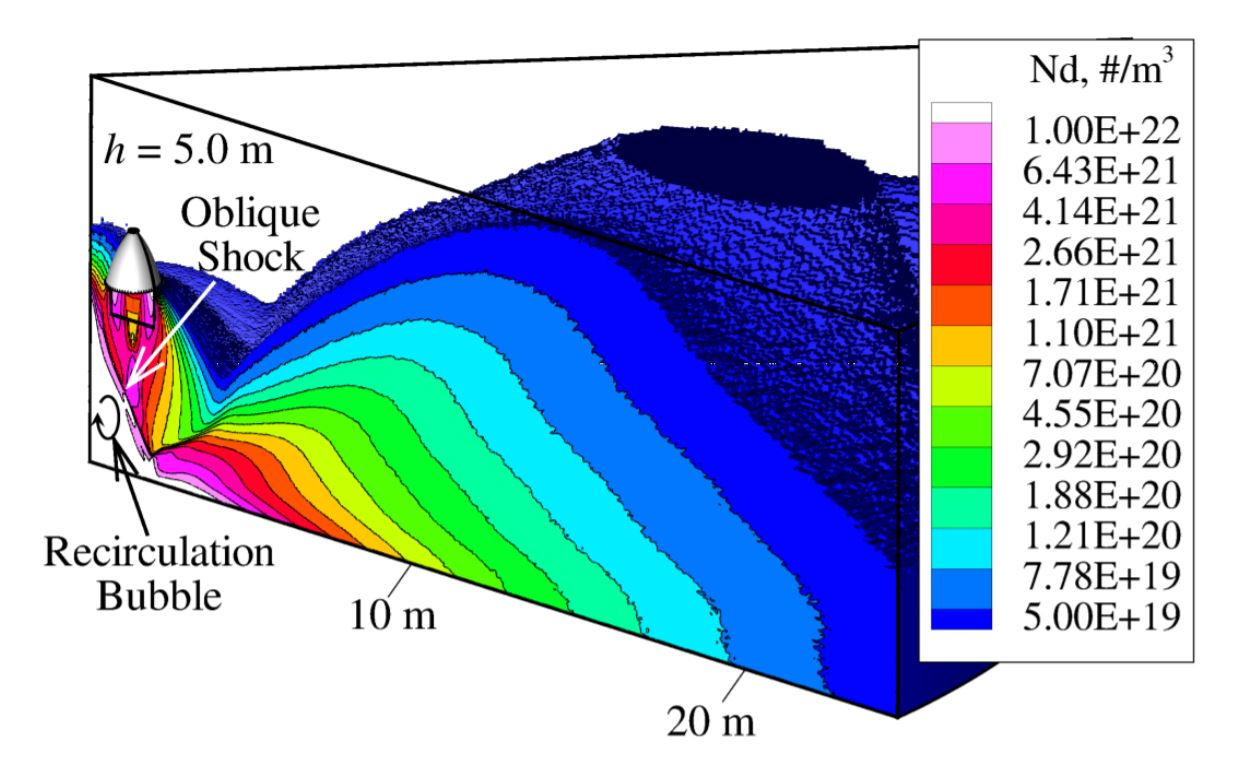
\includegraphics[width=\textwidth]{figures/hover_rocket.JPG}
  \end{minipage} %
  \begin{minipage}[b]{0.49\textwidth}
    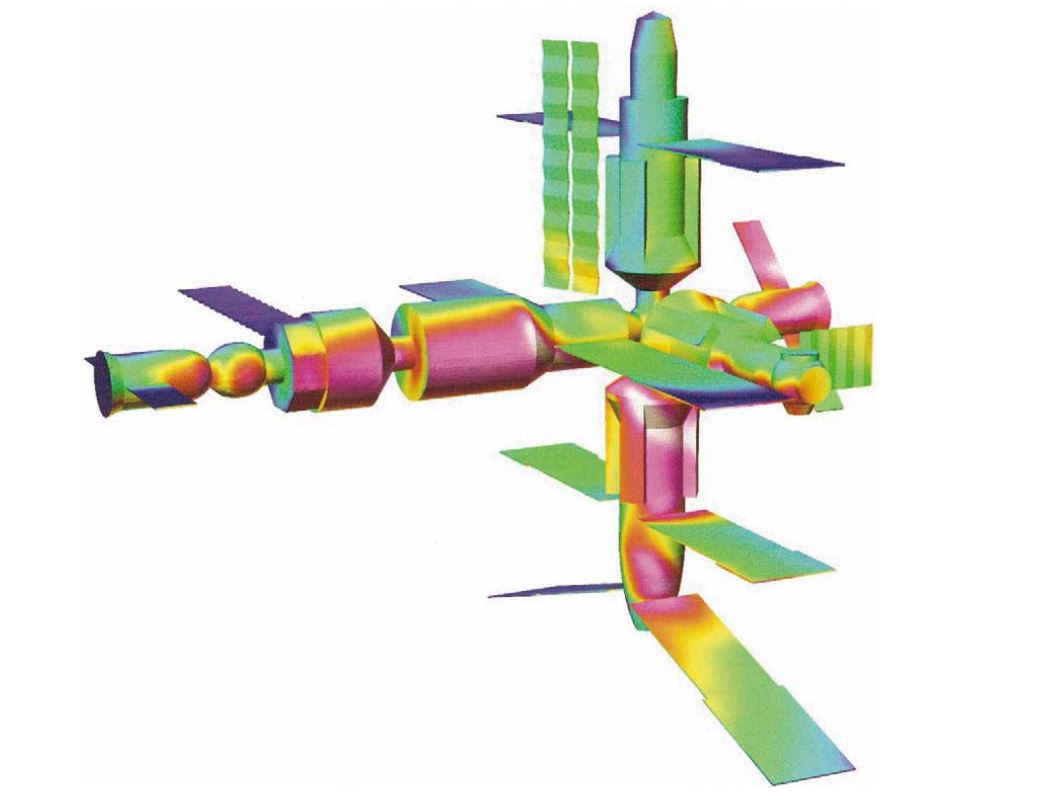
\includegraphics[width=\textwidth]{figures/mir_shuttle.JPG}

  \end{minipage}
  \caption[DSMC Application Examples]{(left) A rocket lander hovering 5 m above the surface \cite{hover_rocket}. (right) Predicted surface pressure on Mir from the Space Shuttle RCS during docking \cite{mir_shuttle}.}
  \label{fig:dsmc_application}
\end{figure}

\indent DSMC fits into an important gap in fluid simulation methods. It is a particle-based method, which allows it to accurately model high Knudsen number simulations in cases when continuum codes break down. Yet it does this while remaining based on statistical sampling and therefore allows critical computation time-saving mathematics and algorithms to allow DSMC to be on par with legacy continuum methods. DSMC simulates many super-particles in a domain, each of which is comprised of millions of physical particles. DSMC then uses statistics to determine collisions and surface interactions. The super-particles allow for a greater range of high Knudsen number scenarios to be simulated which is of particular interest in astronautics where Knudsen numbers are traditionally high. As seen in Figure \ref{fig:dsmc_application}, DSMC is now used for many important aerospace analysis tasks. \par


\indent Unfortunately, DSMC alone does not account for a large area of aerospace research: plasma. Plasma exists when there are a large number of ions and enough high-energy electrons to keep ionizing the gas. As seen in Table \ref{tab:plasma}, plasma can exist in many various situations and environments. Even commonplace things like candle flames or lightning bolts contain some plasma. Two large areas of aerospace research which take place within a plasma environment are atmospheric re-entry and electric propulsion. Both exist in a high Knudsen number environment but include charged particles. Therefore, while DSMC would be well-suited for the situation, it is not able to model the charged particles in these situations. \par




\indent Plasma is comprised, on average, of equal parts of negative electrons and positive ions, otherwise known as quasi-neutrality. However, there can be systematic (electric thruster) or random (solar wind) fluctuations that cause a local net charge. This fact means that the plasma can create electric forces, which in turn affect the charged particles in a plasma. DSMC cannot simulate charged particle flows because it only has mechanisms for collisional velocity updates. DSMC does not have a mechanism to calculate the electric force and update the particles velocities. This is where the Particle-In-Cell (PIC) method applies. \par


\begin{table}
\caption[Various Plasmas]{Various Plasmas \cite{plasma_table}. \(n\) - Number Density, \(T\) - Plasma Temperature}
\label{tab:plasma}
\vspace{0.3cm}
\begin{center}
\begin{tabular}{|lll|}
\hline
Plasma Type          & n (cm\textsuperscript{-3}) & T (eV)                  \\ \hline
Interstellar gas     & 1                        & 1                     \\
Solar Corona         & 10\textsuperscript{3}    & 1                     \\
Hot Plasma           & 10\textsuperscript{14}   & 10\textsuperscript{2} \\
Thermonuclear Plasma & 10\textsuperscript{15}   & 10\textsuperscript{4} \\
Laser Plasma         & 10\textsuperscript{20}   & 10\textsuperscript{2} \\ \hline
\end{tabular}
\end{center}
\end{table}

\indent The PIC method is a standard method to calculate the force on electrically charged particles in a particle type model. It is based on a mesh system comprised of nodes, upon which field calculations are made. The mathematics of charged particle forces in terms of PIC will be discussed in Chapter \ref{chap:charge}. PIC, however, does not account for collisions between particles. To accurately model a plasma for aerospace research, collisions between particles need to be taken into account. This naturally leads to the necessity for a DSMC-PIC hybrid method. A single mesh can be used for calculating collisions and macro-properties through DSMC as well as being used to calculate the fields in the domain and how they affect the particle's velocities with PIC. This allows for a program which can simulate a greater range of scenarios. However, it may be necessary with more complicated simulations to have different mesh sizes for the DSMC portion from the PIC portions. \par


\indent One scenario within aerospace research for which a DSMC-PIC simulation is optimal is electric propulsion. There are three main methods of spacecraft propulsion: chemical, cold gas, and electric. Chemical is the classic rocket engines used to put spacecraft and humans into orbit. Cold gas is simply expelling pressurized gas to provide thrust. Electric propulsion uses electricity to create more efficient engines for spacecraft. Electric propulsion can either be electrostatic, electrothermal, or electromagnetic. A nearly universal property of electric thrusters is that the exhaust is usually in a plasma state. An electric propulsion engine, in this case an ion engine, is shown in Figure \ref{fig:ion_thruster}. This figure shows the neutral propellant gas being ionized in the chamber, then the ions accelerated out through magnetic grids to create thrust\footnote{A more detailed explanation of ion engines and other information about electric propulsion can be found in Reference \cite{gobel}}. This results in a plasma plume. Since the spacecraft is in space and the thrusters do not expel dense amounts of gas, this plasma fits right into the realm of a DSMC-PIC simulation. Herein this lies the motivation for this thesis. \par


\begin{figure}
    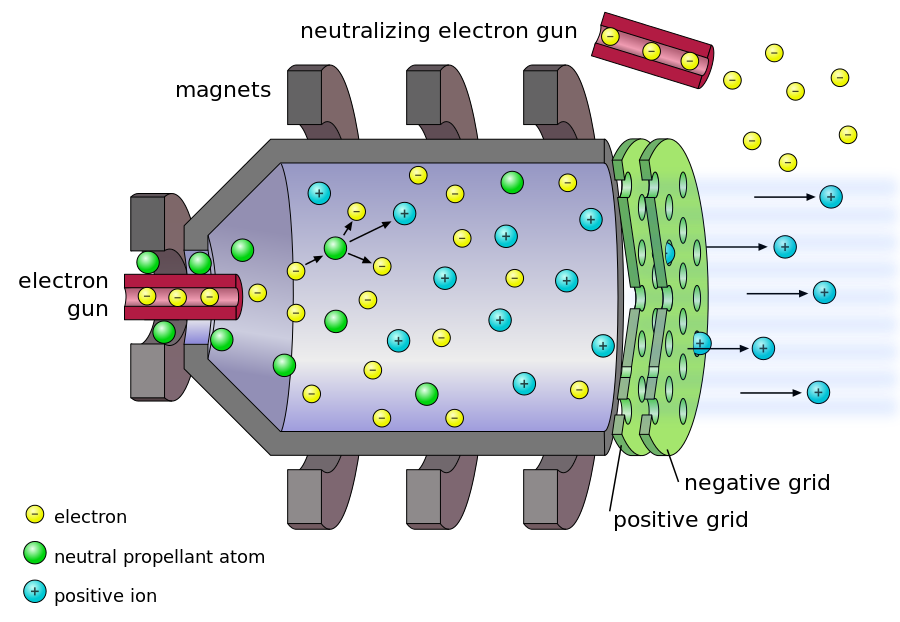
\includegraphics[width=.85\textwidth]{figures/ion_thruster.png}
    \centering
    \caption[Diagram of an Ion Thruster]{Diagram of an Ion Thruster \cite{ion_thruster} }
    \label{fig:ion_thruster}
\end{figure}

%\footnote{By Oona Räisänen - Own work; self made in Inkscape. Based on File:Ion_engine.gif., CC BY-SA 3.0, https://commons.wikimedia.org/w/index.php?curid=20308289}

%\section{Literature Review}


%As discussed above, the DSMC and PIC methods are not new innovations. Neither is the DSMC-PIC combination. Therefore, there are many resources from which to draw important information about algorithms, pitfalls, and challenges of implementing this method. 



\section{Overarching Goal}
This thesis is one of a series of projects. The end goal is to have a Cal Poly homegrown simulation that can simulate an entire electric thruster. While the individual areas of modeling the discharge chamber \cite{discharge} and modeling the plasma plume \cite{justplume} are growing strongly, there is a distinct lack of complete electric thruster models in literature. It is technically possible to simulate the entirety of the thruster in DSMC, but the Knudsen number is so low inside of the thruster that computing a DSMC method would be nearly impossible. A simulation of a full electric thruster requires a continuum simulation for the gas inside the thruster and then a rarefied gas simulation for the exhaust plume where the Knudsen number is higher. In order to model a complete thruster, researchers have compromised by attempting to join together a fluid code and a rarefied gas code. Cal Poly's Aerospace Department is rare in that a fluid code and a rarefied gas code are being developed in the exact same manner from the ground up. Other institutions are also working in this area with success in the initial stages \cite{afrl,afrl_copy}. The early developers and advisors at Cal Poly worked together to establish these codes as being compatible from the beginning. \par

\indent This thesis is the third project of a homegrown DSMC code, code name SINATRA, which will eventually be able to simulate the thruster's plasma exhaust plume. The first three developers worked together in a staggered capacity to build SINATRA up to a working DSMC-PIC code. The first, Galvez, developed the base framework and kinematics \cite{Galvez2018a}. Next Alliston built up the collisions and particle models \cite{mac_thesis}. This thesis adds charged particle simulation capability to SINATRA. Concurrently with this thesis, Gay has been building the fluid side simulation \cite{Gay}. Intentionally, many properties will be common between the codes. They are both written in C++ and are class-based. They share the same process control items, including the execution style, distribution method, and the other systems items shown in Chapter \ref{chap:systems}. They share the same mesh type and input class to help them work together as one simulation. A future project will take both simulations and build the interaction system to connect them across each time-step.
%Is SINATRA a steady state or transient solver?]] 
% Dom - able to be both! depending on output settings and how many times you rerun the same simulation